%%%%%%%%%%%%%%%%%%%%%%%%%%%%%%%%%%%%%%%%%%%%%%%%%%%%%%%%%%%%%%%%%%%%%%%%
%                                                                      %
% LaTeX, FIIW thesis template                                          %
% 28/11/2014 v1.2                                                      %
%                                                                      %
%%%%%%%%%%%%%%%%%%%%%%%%%%%%%%%%%%%%%%%%%%%%%%%%%%%%%%%%%%%%%%%%%%%%%%%%
\documentclass[11pt,a4paper]{report}
% Indien je je thesis recto-verso wil afdrukken gebruik je onderstaande opties i.p.v. bovenstaande
%\documentclass[11pt,a4paper,twoside,openright]{report}

\usepackage[a4paper,left=3.5cm, right=2.5cm, top=3.5cm, bottom=3.5cm]{geometry}
\usepackage[english]{babel}
\usepackage{titlesec}

\usepackage{graphicx}
%\usepackage[latin1]{inputenc}           % om niet ascii karakters rechtstreeks te kunnen inputten
% \usepackage[utf8]{inputenc}            % commentarieer deze regel uit als je utf8 encoded files gebruikt in plaats van latin1
\usepackage[authoryear, round]{natbib}
\usepackage{listings}             		% voor het weergeven van broncode
\usepackage{verbatim}					% weergeven van code, commando's, ...
\usepackage[hidelinks]{hyperref}		% maak PDF van de thesis navigeerbaar without boxes
%\usepackage{hyperref}					% maak PDF van de thesis navigeerbaar
% \usepackage{url}						% URL's invoegen in tekst met behulp van \url{http://}
\usepackage[small,bf,hang]{caption}     % om de captions wat te verbeteren
\usepackage[final]{pdfpages}            % gebruikt voor het invoegen van het artikel in pdf-formaat
\usepackage{pslatex}					% andere lettertype's dan de standaard types
% \usepackage{lipsum}
\usepackage{sectsty}					% aanpassen van de fonts van sections en chapters
%\usepackage[nottoc,numbib]{tocbibind}	% Bibliography mee in de ToC
% \usepackage{tikz}
% \usepackage[table,xcdraw]{xcolor}
% \usepackage{standalone}
\usepackage{enumitem}
% \usepackage{multirow}
% \usepackage{chngpage}
% \usepackage[svgpath=fig/]{svg}
% \usepackage{pdflscape}
% \usepackage{rotating}
\usepackage{newfloat}
% \usepackage{subcaption}
\DeclareFloatingEnvironment[fileext=frm,placement={!ht},name=Listing,within=chapter]{listing}

\setlist{nosep}
%\usetikzlibrary{external}
\usepackage{mdframed}
\usepackage[acronym]{glossaries}
\usepackage{algorithm}
\usepackage{algpseudocode}
% \usepackage{amssymb}% http://ctan.org/pkg/amssymb
\usepackage{pifont}% http://ctan.org/pkg/pifont
\newcommand{\cmark}{\ding{51}}%
\newcommand{\xmark}{\ding{55}}%

\allsectionsfont{\sffamily}
\chapterfont{\raggedleft\sffamily}

% \usepackage{float}                      % De optie H voor de plaatsing van figuren op de plaats waar je ze invoegt. bvb. \begin{figure}[H]
%\usepackage{longtable}					% tabellen die over meerdere pagina's gespreid worden
%\usepackage[times]{quotchap}           % indien je fancy hoofdstuktitels wil
%\usepackage[none]{hyphenat}
%\usepackage{latexsym}
% \usepackage{amsmath}

% MFA: zet zoekpad voor figure
\usepackage{subcaption}
\graphicspath{{fig/}}

\usepackage{fiiw_eng}

%door onderstaande regels in commentaar te zetten, of op false, kan je pagina's weglaten
%bijvoorbeeld het weglaten van een voorwoord, lijst met symbolen, ...
%%%%%%%%%%%%%%%%%%%%%%%%%%%%%%%%%%%%%%%%%%%%%%%%%%%%%%%%%%%%%%%%%%%%%%%%%%%%%%%%%%%%%%%%
%voorwoord toevoegen?
%\acknowledgementspagetrue
\acknowledgements{voorwoord}			%.tex file met daarin het voorwoord

%samenvatting toevoegen
%\summarypagetrue
\summary{samenvatting}					%.tex met daarin de samenvatting

%abstract toevoegen?
\abstractpagetrue
\abstracts{abstract}					%.tex file met daarin het abstract
%lijst van figuren toevoegen?
%\listoffigurespagetrue
%lijst van tabellen toevoegen?
% \listoftablespagetrue
%lijst van symbolen toevoegen?
%\listofsymbolspagetrue
%\listofsymbols{symbolen}				%.tex file met daarin de lijst van symbolen
\listofabbrevspagetrue
\listofabbrevs{abreviations}			%.tex file met daarin de lijst van afkortingen


%informatie over het eindwerk, de promotor, ...
%%%%%%%%%%%%%%%%%%%%%%%%%%%%%%%%%%%%%%%%%%%%%%%
\opleiding{Electronics-ICT}
\afdeling{}

\campus{denayereng} %denayer,denayereng,geel,geeleng,gent,ghenteng,groept,groupteng,brugge,brugeseng

\title{Inverting knowledge graphs back to raw data}
\subtitle{How can we leverage the rules we use to construct knowledge graphs to do the inverse?}
% \author{naam student}
\forenameA{ }
\surnameA{ }

\forenameB{Tijs}
\surnameB{Van Kampen}

\academicyear{2023 - 2024}

\promotorA[Promotor]{Prof dr. ir. Anastasia Dimou}
\promotorB[Co-Promotor]{}

\begin{document}
\selectlanguage{english} % For the English version

\preface 

% \printglossary[type=\acronymtype, title=List of abbreviations, toctitle=List of abbreviations]

\lstset{moredelim=[is][\bfseries]{[*}{*]}}

%%%%%%%%%%%%%%%%%%%%%%%%%%%%%%%%%%%%%%%%%%%%%%%%%%%%%%%%%%%%%%%%%%% 
%                                                                 %
%                            CHAPTER                              %
%                                                                 %
%%%%%%%%%%%%%%%%%%%%%%%%%%%%%%%%%%%%%%%%%%%%%%%%%%%%%%%%%%%%%%%%%%% 

\chapter{Introduction}
\label{chapter:introduction}

The earliest academic definition of a knowledge graph can be found in a 1974 article as \begin{quote}
    A mathematical structure with vertices as knowledge units connected by edges that represent the prerequisite relation \citep{Marchi1974,bergman2019common}
\end{quote} 

The idea of expressing knowledge in a graph structure predates even this definition, with the concept of semantic networks \citep{Richens1956PreprogrammingFM}. % This is in the age of punch card computers, so quite impressive 
However, the term knowledge graph only became well-known after Google announced they were using a knowledge graph to enhance their search engine in 2012 \citep{singhal2012introducing}. 
Knowledge graphs are used to make search engines, chatbots, question-answering systems, etc more intelligent by injecting knowledge into them \citep{SurveyOnKGs}. 

A knowledge graph consists of many connected nodes, where each node is either an entity or a literal. These nodes are connected by edges, where each edge defines a relation between two nodes. \acrfull{rdf} \citep{rdfprimer} is a framework often used to represent knowledge graphs, it uses subject-predicate-object triples to represent the nodes and their edges. Every subject node is either an \acrshort{uri} or a blank node, while the object can be a literal value. The edges are \acrshortpl{uri}. This triple: \texttt{http://example.com/John\_Doe http://schema.org/givenName "John" .} would represent the fact that the entity \texttt{John Doe} has the first name \texttt{John}. Often the predicates are chosen from an ontology/vocabulary, such as schema.org or \acrshort{foaf}. This allows for more interoperability between knowledge graphs, as the same predicates are used to represent the same concepts.

These knowledge graphs are constructed by extracting information from various sources, both unstructured sources such as text (using natural language processing) and (semi-)structured sources such as databases, \acrshort{csv}, \acrshort{xml}, \acrshort{json}, \acrshort{rdf} (using mapping languages). Many mapping languages exist, differing in the way of defining the rules and the target source file format. Some mapping languages use the turtle syntax, while others provide their custom syntax, and others repurpose existing languages like \acrshort{sparql} or \acrshort{shex} \citep{VANASSCHE2023100753}. Some languages are specific to a single source format, such as R2RML(turtle format) \citep{Das:12:RRR} for relational databases, XSPARQL(\acrshort{xquery} format) \citep{Bischof2012} for XML. Others can process multiple formats, such as RML (turtle) \citep{dimou_ldow_2014}, D-REPR (\acrshort{yaml}) \citep{d-repr}, xR2RML (turtle) \citep{xR2RML}, etc. These can handle mapping from multiple sources in different formats.

To achieve the mapping of data these mapping languages use a declarative approach where the user specifies rules describing the desired output knowledge graph, the mapping rules. The implementation then takes care of the logic and transformations behind the mapping. Two ways of mapping exist, materialization and virtualization. Materialization constructs the knowledge graph as a file, which can be loaded into a triple store. Virtualization does not generate the knowledge graph as a file, but instead exposes a virtual knowledge graph, which can be queried as if it were a real knowledge graph. \citep{ontop}.

Creating these mapping rules is often done by hand. Some tools ease the creation process of these mappings, like RMLEditor \citep{heyvaert_jws_2018} which exposes a visual editor, and YARRRML \citep{10.1007/978-3-319-98192-5_40} which allows users to create rules in the user-friendly \acrshort{yaml} which are then compiled to RML rules. 

Retrieving data from a knowledge graph, for consumption by other programs, can be done by querying the knowledge graph using SPARQL \citep{Seaborne:08:SQL}. Using a select query data can be retrieved in a tabular format. A construct query can be used to retrieve the data in RDF format. 

A knowledge graph cannot be converted back to the original data format using the same rules we created it with. As a result any changes we make to the knowledge graph are hard to propagate back. We can not update, expand, or improve the original data using e.g. knowledge graph refining nor can we apply changes to a virtual knowledge graph to change the original data. 

In this work, we seek to answer the question: \textit{How can we extend an existing mapping language like RML or create a new system to construct raw data from knowledge graphs?} We choose to extend the Morph-KGC implementation \citep{arenas2022morph} of \acrshort{rml} \citep{dimou_ldow_2014} as \acrshort{rml}'s end-to-end (from file to knowledge graph) characteristics make it a good candidate for this task. To answer the main research question we need to answer the following sub-questions:
\begin{itemize}
    \item[\textit{RQ1}] \textit{How can we construct the schema of the original data from the mapping rules?}
    \begin{itemize}
        \item We will study each type of source format, as each format has its challenges.
    \end{itemize}
    \item[\textit{RQ2}] \textit{How can we populate the schema with data from the knowledge graph?}
    \begin{itemize}
        \item We will study how we can best retrieve the data, trying different approaches.
    \end{itemize}
\end{itemize}

\section{Thesis outline}
The aim of this thesis is to explore the possibility of inverting knowledge graphs back to their original data format using RML mapping rules, we choose RML as it is well-adopted and has many implementations. To achieve this we will take a closer look at the technologies used like RDF, SPARQL, and RML in chapter \ref{chapter:related_work}. 
In chapter \ref{chapter:implementation} a closer look will be taken at our implementation of the inversion algorithm. We will look at the algorithm itself, and the implementation details. 
In chapter \ref{chapter:evaluation} an evaluation of our implementation using various benchmarks will be done. For basic testing, we use a subset of the RML test cases, which are designed to test the conformance of tools to the RML specification. For more advanced testing we will use various benchmarks simulating real-life use cases like LUBM4OBDA, GTFS-Madrid-Bench, and SDM-Genomic-dataset. Finally in chapter \ref{chapter:conclusion} we will conclude this thesis, and look at possible future work.

%%%%%%%%%%%%%%%%%%%%%%%%%%%%%%%%%%%%%%%%%%%%%%%%%%%%%%%%%%%%%%%%%%% 
%                                                                 %
%                            CHAPTER                              %
%                                                                 %
%%%%%%%%%%%%%%%%%%%%%%%%%%%%%%%%%%%%%%%%%%%%%%%%%%%%%%%%%%%%%%%%%%% 

\chapter{Related work}
\label{chapter:related_work}

In this chapter, we discuss the various technologies related to this thesis. We begin by discussing the semantic web and build from there to technologies used within its ecosystem like \acrshort{rdf}, \acrshort{sparql}, and mapping languages. We finish by discussing the current state of the art in updating or creating the original data source from a knowledge graph.

\section{Semantic Web}
Tim Berneers-Lee envisioned a version of the web that would also be understandable by machines, and thus the semantic web was born. It is not designed as a separate entity to the web, but instead as an extension, designed not for use by humans but rather computer 'agents'. It is designed with existing technologies like \acrshort{xml}, \acrshortpl{uri} and \acrshort{rdf}. Even ontologies, a key component of the semantic web, are not a new concept but rather co-opted from the field of philosophy. \citep{thesemanticweb}

\section{RDF}
\acrfull{rdf} was originally designed as a data model for metadata but has since been extended to be a general-purpose framework for graph data. RDF is a directed graph, where the nodes represent entities, and the edges represent relations between these entities. This graph is built up from triples, which connect a subject and an object using a predicate as shown in figure \ref{fig:rdf_triple}.

\begin{figure}
    \centering
    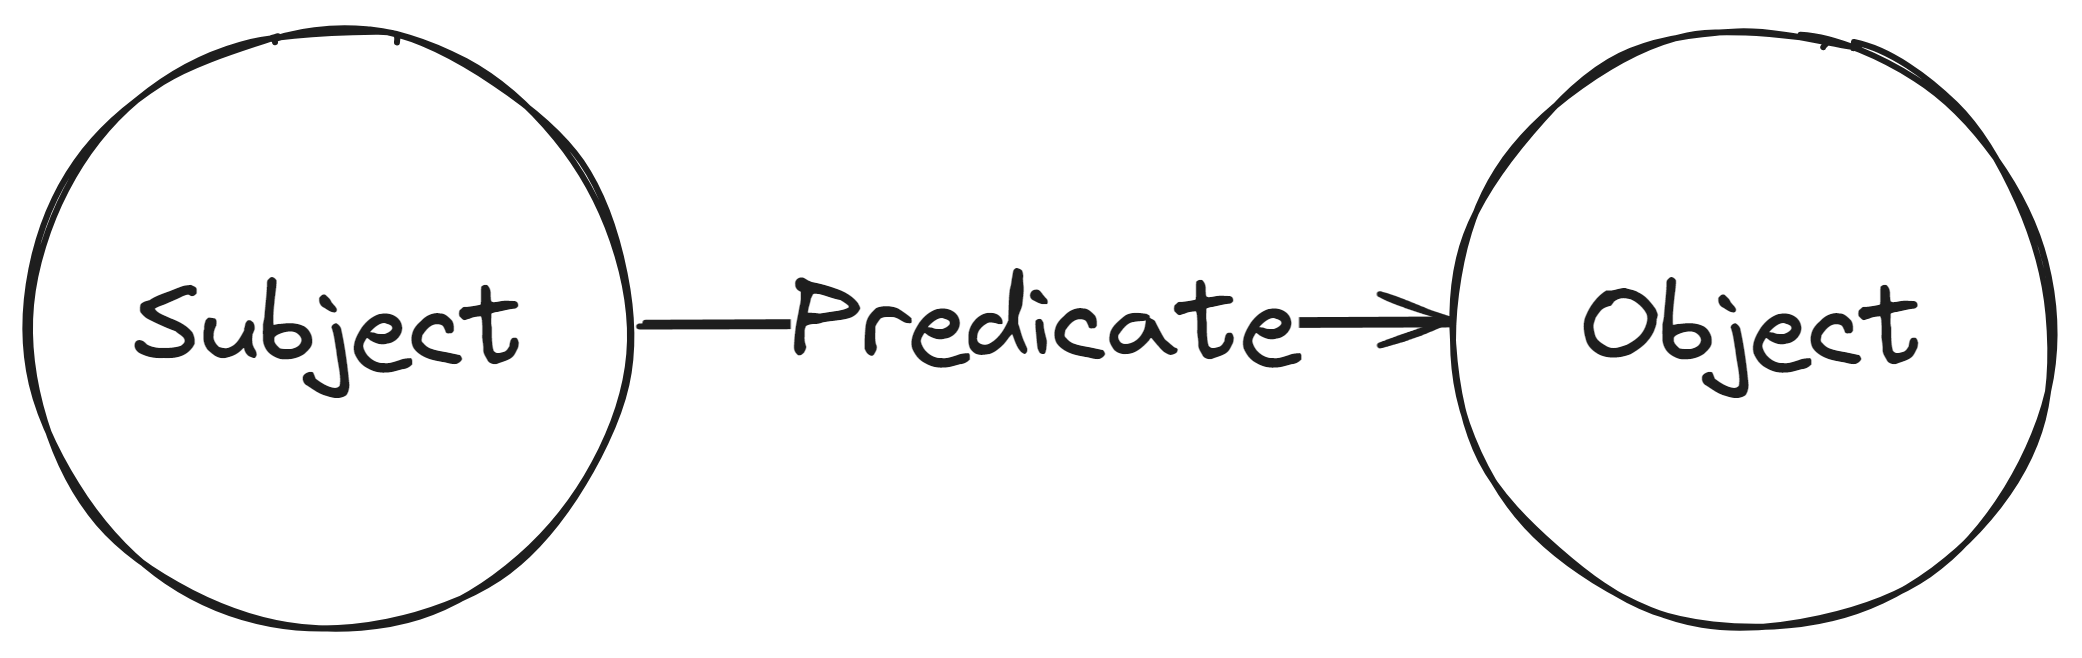
\includegraphics[width=0.5\textwidth]{Chapter2/SPO}
    \caption{An RDF triple}
    \label{fig:rdf_triple}
\end{figure}

The subject must always be an entity, which can either be represented by an \acrshort{uri} or be a blank node. The predicate must be an \acrshort{uri}, and the object can be either an \acrshort{uri}, a blank node, or a literal. \citep{rdfprimer}

% less than character: \textless
% greater than character: \textgreater

\begin{figure}[]
    \begin{tabular}{lll}
        \textbf{Subject}                                   & \textbf{Predicate}                                 & \textbf{Object}                                     \\
        \textless http://example.com/De\_Nayer\textgreater & \textless https://schema.org/location\textgreater  & \textless http://example.com/Mechelen\textgreater . \\
        \textless http://example.com/r0785695\textgreater  & \textless https://schema.org/givenName\textgreater & ``Tijs" .
    \end{tabular}
    \caption{Example of RDF triples}
    \label{fig:rdf_triples_table}
\end{figure}

A \acrshort{uri} is a unique identifier for a resource on the web. Unlike a normal \acrshort{url}, it does not have to point to a network location, but can also be used to identify a person, a location, a concept, etc. \citep{rdfprimer}. In \acrshort{rdf} the \acrshort{uri} is purely used for identifying resources. As such, unlike in HTML where certain conventions are expected, there are no conventions for \acrshortpl{uri} in \acrshort{rdf}. An example of this can be seen in figure \ref{fig:rdf_triples_table}, the example subjects share the same domain but this does not imply that they are closely related, or even related at all. \acrshortpl{uri} are extended to \acrshortpl{iri} to allow for a wider range of characters. Except for allowing Unicode characters, \acrshortpl{iri} are identical to \acrshortpl{uri} so little distinction is made between the two in this thesis.

A blank node is a node that is not identified by a \acrshort{uri}. It is used to represent an anonymous resource that can't be or has no reason to be uniquely identified. For example, the address of student r0785695 in figure \ref{fig:blank_node} is only pertinent to the student and thus does not need to be uniquely identified. A blank node is serialized as \texttt{\_:name}, where name is a unique identifier for the blank node. This identifier is only unique within the document, and thus can't be used to refer to the blank node from outside the document. \citep{rdfprimer}

\begin{figure}[]
    \begin{tabular}{lll}
        \textbf{Subject}    & \textbf{Predicate}   & \textbf{Object}                                      \\
        ex:student/r0785695 & schema:address       & \_:addrr0785695                                      \\
        \_:addrr0785695     & schema:postalCode    & ``2800"\textasciicircum \textasciicircum xsd:integer \\
        \_:addrr0785695     & schema:streetAddress & ``Gentsesteenweg XXXX"@nl
    \end{tabular}
    \caption{Example of a blank node and prefix notation}
    \label{fig:blank_node}
\end{figure}

A literal is a value, e.g. a string, integer, or date. This value can be typed, e.g. a string can be typed as a date, or untyped. A string can also have a language tag, which is used to indicate the language of the literal.

RDF is only a framework, and as such does not define any serialization syntax. There are however a few common serialization standards for example RDF/XML, Turtle, N-Triples, and JSON-LD.

\subsection{Turtle}
Turtle, or Terse RDF Triple Language, is a human-readable serialization format for \acrshort{rdf}. It is the most used serialization format for \acrshort{rdf}, and is used in many tools and specifications.
In its simplest form turtle consists of triple statements, sequences of subject-predicate-object separated by spaces and terminated by a dot. An example of this can be seen in listing \ref{lst:basic_turtle_example}. This is very verbose, but Turtle offers many features to make it more concise. Below is a list of some of these features and, if possible, how they can be used to make the example more concise.
\begin{itemize}
    \item \textbf{Prefix notation} allows us to shorten \acrshortpl{uri} by defining a prefix.
          \begin{itemize}
              \item Using \texttt{@prefix schema: <https://schema.org/>} allows us to shorten \break\texttt{https://schema.org/Person} to \texttt{schema:Person}
          \end{itemize}
    \item \textbf{Base prefix} allows us to shorten \acrshortpl{uri} by defining a base \acrshort{uri}.
          \begin{itemize}
              \item Using \texttt{@base <http://example.com/>} allows us to shorten \break\texttt{http://example.com/r0785695} to \texttt{r0785695}
          \end{itemize}
    \item \textbf{Predicate lists} allow us to shorten multiple triples with the same subject to a list of predicates.
          \begin{itemize}
              \item Our example only has two subjects, we can split their predicates with \texttt{;} instead of repeating the subject.
          \end{itemize}
    \item \textbf{Object lists} allow us to shorten multiple triples with the same subject and predicate to a list of objects.
          \begin{itemize}
              \item \texttt{r0785695} is both a Person and a Student, so we can split the objects with \texttt{,} instead of repeating the subject and predicate.
          \end{itemize}
    \item \textbf{Literals} allow identifying values, e.g. strings, integers, dates, etc. with a datatype or language tag.
    \item \textbf{Blank nodes} allow us to define anonymous resources by using the \texttt{\_:} prefix.
          \begin{itemize}
              \item The address of \texttt{r0785695} is only relevant to \texttt{r0785695}, so we can define it as a blank node instead of using a \acrshort{uri}, this shortens \texttt{<http://example.com/addrr0785695>} to \texttt{\_:addrr0785695}. While not exactly the same, functionally it is equivalent as we do not expect addresses to be addressed outside of the context of a person.
          \end{itemize}
    \item \textbf{Unlabeled blank nodes} allow us to define anonymous resources without explicitly defining an identifier by using the [] notation instead of \texttt{\_:name}.
          \begin {itemize}
    \item As we do not need to refer to \texttt{\_:addrr0785695} from outside \texttt{r0785695}, we can use an unlabeled blank node and include it in \texttt{r0785695} instead of a labeled blank node.
\end{itemize}
\item \textbf{Collections} allow us to define a list of nodes by using the () notation.
\end{itemize}
The example in listing \ref{lst:basic_turtle_example} can be rewritten using these features, as shown in listing \ref{lst:basic_turtle_example_concise}.


\begin{lstlisting}[caption={Basic naive turtle document}, label={lst:basic_turtle_example}, captionpos=b, breaklines=true, basicstyle=\small]
    <http://example.com/r0785695> <http://www.w3.org/1999/02/22-rdf-syntax-ns#type> <http://schema.org/Person> .
    <http://example.com/r0785695> <http://www.w3.org/1999/02/22-rdf-syntax-ns#type> <http://schema.org/Student> .
    <http://example.com/r0785695> <http://schema.org/givenName> "Tijs" .
    <http://example.com/r0785695> <http://schema.org/familyName> "Van Kampen" .
    <http://example.com/r0785695> <http://schema.org/address> <http://example.com/addrr0785695> .
    <http://example.com/addrr0785695> <http://schema.org/postalCode> "2800"^^<http://www.w3.org/2001/XMLSchema#integer> .
    <http://example.com/addrr0785695> <http://www.w3.org/1999/02/22-rdf-syntax-ns#type> <http://schema.org/PostalAddress> .
    <http://example.com/addrr0785695> <http://schema.org/streetAddress> "Gentsesteenweg XXXX"@nl .
    <http://example.com/addrr0785695> <http://schema.org/addressCountry> "Belgium" .
\end{lstlisting}

\begin{lstlisting}[caption={Basic turtle document using turtle features}, label={lst:basic_turtle_example_concise}, captionpos=b, breaklines=true]
    @prefix schema: <https://schema.org/> .
    @prefix xsd: <http://www.w3.org/2001/XMLSchema#> .
    @base <http://example.com/> .
    <r0785695> a schema:Person, schema:Student ;
        schema:givenName "Tijs" ;
        schema:familyName "Van Kampen" ;
        schema:address [
            a schema:PostalAddress ;
            schema:postalCode "2800"^^xsd:integer ;
            schema:streetAddress "Gentsesteenweg XXXX"@nl ;
            schema:addressCountry "Belgium"
        ] .
\end{lstlisting}


\section{SPARQL}
\acrfull{sparql} is the \acrshort{w3c} standard query language for \acrshort{rdf}. It is the main way to query \acrshort{rdf} data and shows many similarities to SQL. \acrshort{sparql} queries mostly consist of a pattern of triples, which are matched against the \acrshort{rdf} graph, a basic example can be found in listing \ref{lst:sparql_select_query}. Querying is very feature-rich, with support for aggregation, subqueries, negation, regex, string manipulation, etc. It also supports different return types, federated queries, entailment, etc \citep{SPARQL1.1QL}. Aside from the query protocol it also defines the graph store protocol, which can be used to manipulate graph databases directly \citep{SPARQL1.1}.

\begin{lstlisting}[language=SPARQL, caption={Example of a basic \acrshort{sparql} SELECT query}, label={lst:sparql_select_query}, captionpos=b]
    PREFIX schema: <https://schema.org/>
    SELECT ?name ?address
    WHERE {
        ?student schema:givenName ?name .
        ?student schema:address ?address .
    }
\end{lstlisting}

\section{Mapping languages}
Mapping languages are used to define a mapping between a source and a target. The target in the context of linked data is of course \acrshort{rdf}, with the source being any structured data source. Some mapping languages exist for a single source, e.g. \acrfull{r2rml} for relational databases, \acrfull{xsparql} for \acrshort{xml}, etc. Others are more general purpose, e.g. \acrfull{rml} and \acrfull{d2rml}.
We will discuss both \acrshort{r2rml} and \acrshort{rml} in more detail, as one extends the other. \acrshort{r2rml} is significant as it is the most widely used mapping language, as it supports virtualization \textit{ontop} of databases.\acrshort{rml} extends \acrshort{r2rml} with more features and source types making it one of the more feature-rich general mapping languages, as such it is the mapping language we will use in our implementation.
Most \acrshort{rml} implementations also support \acrshort{r2rml}, as \acrshort{rml} is a nearly superset of \acrshort{r2rml}.

\subsection{\acrshort{r2rml}}
\acrfull{r2rml} is a mapping language for mapping relational databases to \acrshort{rdf}. As opposed to \acrfull{dm}, which results in a direct mapping from the relational database to \acrshort{rdf} without any changes to structure or naming, \acrshort{r2rml} allows for more flexibility. R2RML mappings consist of zero or more TriplesMaps, which are used to map a table to \acrshort{rdf}. A TriplesMap consists of a logical table, a subject map, and one or more \acrfullpl{pom}.

The logical table is used to define the table that is being mapped, with each row in the table being mapped to a subject and its corresponding \acrshortpl{pom}. It is possible to create a view of a table by using a SQL query, and then map this view. This allows for more complex mappings, e.g. mapping a join of two tables or a computed column.
% Could add this, but as we don't actually support R2RML in our implementation for now this is not really relevant
% An example of this can be seen in listing \ref{lst:r2rml_mapping_view}.

% \begin{lstlisting}[caption={Example of an \acrshort{r2rml} mapping with a view. Snippet from \citep{r2rml}}, label={lst:r2rml_mapping_view}, captionpos=b] 
%     <#TriplesMap1>
%     rr:logicalTable [ rr:sqlQuery """
%         SELECT EMP.*, (CASE JOB
%             WHEN 'CLERK' THEN 'general-office'
%             WHEN 'NIGHTGUARD' THEN 'security'
%             WHEN 'ENGINEER' THEN 'engineering'
%         END) ROLE FROM EMP
%         """ ];
%     rr:subjectMap [
%         rr:template "http://data.example.com/employee/{EMPNO}";
%     ];
%     rr:predicateObjectMap [
%         rr:predicate ex:role;
%         rr:objectMap [ rr:template "http://data.example.com/roles/{ROLE}" ];
%     ].
% \end{lstlisting}

Each of the SubjectMap, PredicateMap, ObjectMap, (and GraphMap) is a subclass of TermMap, which is a function that generates an \acrshort{rdf} term. The map type can be constant, template, or column. The resulting term is then used as the subject, predicate, object, or graph of the triple. The termType of the map determines the type of the term, which can be \acrshort{iri}, blank node, or literal. If the termType is literal, optionally the datatype or language can be added. Following the \acrshort{rdf} specification, not all combinations of termType and map are possible, this is shown in table \ref{tab:termType_map_combinations}. The object map has an additional subclass, a reference object map, in which we refer to another TriplesMap. Using a reference map we can map a foreign key to the subject of another TriplesMap, with a join condition. \citep{r2rml}

\begin{table}[h]
    \begin{tabular}{|l|l|l|l|l|}
        \hline
        \textbf{TermType} & \textbf{Subject} & \textbf{Predicate} & \textbf{Object} & \textbf{Graph} \\ \hline
        IRI               & \cmark           & \cmark             & \cmark          & \cmark         \\ \hline
        Blank node        & \cmark           & \xmark             & \cmark          & \cmark         \\ \hline
        Literal           & \xmark           & \xmark             & \cmark          & \xmark         \\ \hline
    \end{tabular}
    \caption{Possible combinations of TermType and Map type}
    \label{tab:termType_map_combinations}
\end{table}

A constant value is a fixed value, e.g. a \acrshort{uri} or a string. A template is a string with placeholders, which are replaced by values from the logical row. A column is the value of a column in the logical row.

\begin{lstlisting}[language=XML, caption={Example of an \acrshort{r2rml} mapping}, label={lst:r2rml_mapping}, captionpos=b]
@prefix rr: <http://www.w3.org/ns/r2rml#>.
@prefix ex: <http://example.com/ns#>.

<#TriplesMap1>
    rr:logicalTable [ rr:tableName "EMP" ];
    rr:subjectMap [
        rr:template "http://data.example.com/employee/{EMPNO}";
        rr:class ex:Employee;
    ];
    rr:predicateObjectMap [
        rr:predicate ex:id;
        rr:objectMap [ rr:column "EMPNO"; rr:datatype xsd:positiveInteger ].
    ].
\end{lstlisting}

\subsection{\acrshort{rml}}
\acrfull{rml} is a mapping language for mapping any (semi-)structured data source to \acrshort{rdf}. It is a generalization of \acrshort{r2rml} and as such supports all the features of \acrshort{r2rml}. It extends \acrshort{r2rml} by extending database-specific features to make them more general. The differences in usage can be seen in table \ref{tab:r2rml_rml_differences}.

\begin{table}[]
    \begin{tabular}{|ll|ll|}
        \hline
        \multicolumn{2}{|c|}{R2RML} & \multicolumn{2}{c|}{RML}                                                                    \\ \hline
        Logical Table (database)    & \texttt{rr:logicalTable} & Logical Source               & \texttt{rml:logicalSource}        \\ \hline
        Table Name                  & \texttt{rr:tablename}    & URI (pointing to the source) & \texttt{rml:source}               \\ \hline
        column                      & \texttt{rr:column}       & reference                    & \texttt{rml:reference}            \\ \hline
        (SQL)                       & \texttt{rr:SQLQuery}     & Reference Formulation        & \texttt{rml:referenceFormulation} \\ \hline
        per row iteration           &                          & defined iterator             & \texttt{rml:iterator}             \\ \hline
    \end{tabular}
    \caption{Differences between \acrshort{r2rml} and \acrshort{rml}}
    \label{tab:r2rml_rml_differences}
\end{table}

\acrshort{rml} uses the same structure as \acrshort{r2rml}, with TriplesMaps consisting of a logical source, a subject map, and zero or more \acrshortpl{pom}. All the changes relate to the logical source. Whereas in \acrshort{r2rml} the source is always a database, from which we select a table or view, in \acrshort{rml} the source can be one of many different source types like \acrshort{xml}, \acrshort{json}, \acrshort{csv}, etc. Where in \acrshort{r2rml} we simply iterate over the rows of a table, in \acrshort{rml} we can have a source without an implicit iteration pattern, and as such we need to define an iterator.

% \section{if meaningful: provenance}
% provenance could be interesting but is not mainstream enough to use on a larger scale. (-yet? Maybe in future work add a reference)

\section{State of the art}
The state of the art in updating or creating the data source from a knowledge graph can be split in two categories, depending on the methodology used. The first methodology applies to virtualization, where the data is exposed as a virtual knowledge graph over the source data. The other methodology is for materialized knowledge graphs, where the knowledge graph is created as a file that can be loaded into a triple store. We will discuss the state of the art in both methodologies, concluding with the relevance of this work.

\subsection{Virtualization}
Virtualization is the process of exposing a virtual knowledge graph over the source data. This virtual knowledge graph can be queried as if it were a real knowledge graph. To achieve this mappings are used to translate queries over the knowledge graph to queries over the source data.

This is most commonly used to expose a database as a virtual knowledge graph. This way an organization can expose a knowledge graph without having to completely transition to a new system. Most implementations of virtualization layers are read-only though, as the translation of SELECT queries is relatively easy but translating INSERT, DELETE or DELETE/INSERT (update) queries is much less straightforward, or even impossible in many cases. Though propagating changes trough the virtualization layer to the source data could be a big part of the linked data lifecycle, related work on this is scarce. In both ``SPARQL Update queries over R2RML mapped data sources" \citep{unbehauen-k-2017--sparqlUpdate} and ``Practical Update Management in Ontology-Based Data Access" \citep{practical_update_management_in_ontology_based_data_access} the authors propose a similar way of handling updates. Compatible updates are propagated to the source data, while incompatible updates(updates which can not be translated back to the source because of conflicts) are held in an 'overflow' triple store. Further changes may make the incompatible updates compatible, at which point they too are propagated to the source data. Larger changes affecting the general structure of the data are not stored, but instead the mapping is updated to reflect the new structure. The handling of updates is shown in figure \ref{fig:virtualization_update}.

\begin{figure}
    \centering
    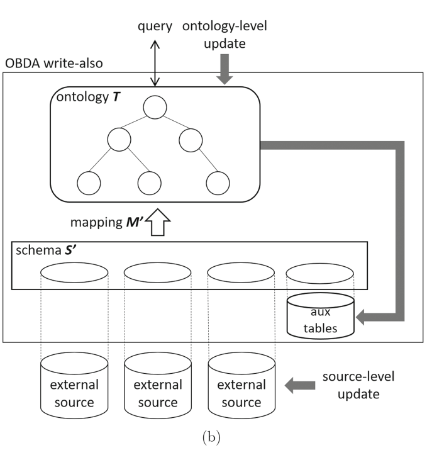
\includegraphics[width=0.6\textwidth]{Chapter2/Write-also_ODBA_architecture.png}
    \caption{Propagating changes in a virtualization layer \citep{unbehauen-k-2017--sparqlUpdate} }
    \label{fig:virtualization_update}
\end{figure}

\subsection{Materialization}
Materialization is the process of creating a knowledge graph as a file that can be loaded into a triple store. The knowledge graph is then loaded into a dedicated triple store for querying. This method benefits from increased performance, at the cost of having the knowledge graph not in sync with the source data.

Materialization allows for a wider range of source formats, as the knowledge graph can be created from any structured data source. This is especially useful when the source data is not easily queryable, e.g. when the source data is a \acrshort{csv}, \acrshort{xml}, or \acrshort{json} file. For knowledge graphs created from structured data sources, use cases exist for propagating changes back to the original data source. This is not done using a direct update (as the source data is not directly connected to the knowledge graph), but by creating a new version of the source data. This process is called lowering. Below we discuss some of the state of the art in lowering.

\subsubsection{\acrshort*{xsparql}}
\acrshort{xsparql} is a mapping language that allows for the transformation of \acrshort{xml} to and back from \acrshort{rdf}. It expands XQUERY with SPARQL-like syntax, structure and features. Its predecessors would do lifting by querying the source \acrshort{xml} using \acrshort{xquery} to transform it into the \acrshort{xml} serialization of \acrshort{rdf}, while lowering was done using XSLT to do the inverse. Using its combined vocabulary \acrshort{xsparql} simplifies lifting and lowering, using a single language for both and having the ability to target the turtle serialization \citep{xsparql}. An example lifting and lowering query can be found in listing \ref{lst:xsparql_lifting} and listing \ref{lst:xsparql_lowering} respectively.

\begin{lstlisting}[caption={Example of \acrshort{xsparql} lifting}, label={lst:xsparql_lifting}, captionpos=b, basicstyle=\small]
declare namespace foaf="http://xmlns.com/foaf/0.1/";
declare namespace rdf="http://www.w3.org/1999/02/22-rdf-syntax-ns#";
let $persons := //*[@name or ../knows]
return

for $p in $persons
let $n := if( $p[@name] )
            then $p/@name else $p
let $id := count($p/preceding::*)
            +count($p/ancestor::*)
where
    not(exists($p/following::*[
        @name=$n or data(.)=$n]))
construct {
    [*_:b{$id} a foaf:Person;*]
                [*foaf:name {data($n)}.*]
    {
        for $k in $persons
        let $kn := if( $k[@name] )
                    then $k/@name else $k
        let $kid := count($k/preceding::*)
                    +count($k/ancestor::*)
        where
            $kn = data(//*[@name=$n]/knows) and
            not(exists($kn/../following::*[
                @name=$kn or data(.)=$kn]))
        construct {
        [*_:b{$id} foaf:knows _:b{$kid}.*]
        [*_:b{$kid} a foaf:Person.*]
        }
    }
}
\end{lstlisting}

\begin{lstlisting}[caption={Example of \acrshort{xsparql} lowering}, label={lst:xsparql_lowering}, captionpos=b, basicstyle=\small]
<relations>{
    for $Person $Name from <relations.rdf>
    where {$Person foaf:name $Name}
    order by $Name
    return
        <person name="{$Name}">{
            for $FName from <relations.rdf>
            where {
                $Person foaf:knows $Friend.
                $Person foaf:name $Name.
                $Friend foaf:name $Fname. }
            return
            <knows>{$FName}</knows>
        }</person>
}</relations>
\end{lstlisting}


\subsubsection{POSER: A Semantic Payload Lowering Service \citep{poser}}
POSER(Payload lOwering SERvice) is a service that lowers \acrshort{rdf} to \acrshort{json}. To achieve this a mapping is created in two parts: first the source patterns are defined from which to extract the data, then the json structure is defined. The mapping is written in turtle, using a custom json ontology describing the json structure. A proof of concept implementation was made, but never got out of the prototype phase. It also only handles direct literal types, more complex composite values that are generated from templates are not supported. An example mapping is shown in listing \ref{lst:poser_mapping}.

\begin{lstlisting}[caption={Example of a POSER mapping}, label={lst:poser_mapping}, captionpos=b, basicstyle=\small]
@prefix ctd: <http://connectd.api/> .
@prefix onto: <http://ontodm.com/OntoDT#> .
@prefix iots: <http://iotschema.org/> .
@prefix json: <http://some.json.ontology/> .
@prefix xsd: <http://www.w3.org/2001/XMLSchema#> .
@prefix time: <https://www.w3.org/TR/2020/CR-owl-time-20200326/> .

# Which inputs to expect and to start mapping from
json:InputDataType {
    json:EntryPoint a iots:TimeSeries;
        iots:providesTemperatureData iots:TemperatureData;
        iots:providesTimeData iots:TimeData .

    iots:TemperatureData iots:numberDataType iots:Number .
    iots:TimeData  time:dateTime iots:Number .
}

#Semantic description of the json objects to be found in the expected API

json:ApiDescription {
    ctd:JsonModel json:hasRoot ctd:Node .

    ctd:TemperatureValue a json:Number ;
        json:key "value"^^xsd:string ;
        json:dataType iots:TemperatureData .

    ctd:TimeStamp a json:String ;
        json:key "timestamp"^^xsd:string ;
        json:dataType iots:TimeData .

    ctd:Node a json:Object;
        json:key "node"^^xsd:string ;
        json:value ctd:TimeStamp, ctd:TemperatureValue ;
        json:dataType iots:TimeSeries .

    ctd:Edges a json:Array	;
        json:key "edges"^^xsd:string ;
        json:value ctd:Node .
}
\end{lstlisting}

\subsection{Relevance}
As shown in this section the state of the art in updating the source in virtualization is pretty mature, only limited by fundamental limitations. It is however limited to databases. To work with other (semi-)structured data sources materialization is needed. For materialization the state of the art is much more limited. Though methods exist to lower \acrshort{rdf} to other formats, each method is intimately linked to a source type. The mappings are also unidirectional, even \acrshort{xsparql} which offers both lifting and lowering requires a separate mapping for each.

Our work expands RML, which can map from any structured data source to \acrshort{rdf}, with the ability to lower the \acrshort{rdf} back to the original source. We use a single mapping to do both lifting and lowering, as information on where to find the data during lifting can also be used to find where to put the data during lowering. This makes our work unique in the field of lowering \acrshort{rdf} to other formats.

As the state of the art is the most limited for sources to which only materialization applies, this is where our work is most relevant. As such we choose to focus our implementation on this domain. However, the design and concept of our work can be applied to any structured data source, including database updates over a virtual graph.


%%%%%%%%%%%%%%%%%%%%%%%%%%%%%%%%%%%%%%%%%%%%%%%%%%%%%%%%%%%%%%%%%%% 
%                                                                 %
%                            CHAPTER                              %
%                                                                 %
%%%%%%%%%%%%%%%%%%%%%%%%%%%%%%%%%%%%%%%%%%%%%%%%%%%%%%%%%%%%%%%%%%% 
\chapter{Implementation}
\label{chapter:implementation}
In this chapter we present the design and implementation of the proposed system. The design and any of its components are not bound to any specific technology, as such they can be implemented using any programming language, framework or mapping language. For the implementation we first present the general setup of the environment. We then present the implementation of the data retrieval. Lastly we present some implementations of template creation and filling.

\section{System Design}
The system we propose is a pipeline that takes as input a knowledge graph and set of mapping rules and outputs the source files from which it would have been constructed. It has the advantage of being very modular, consisting of just data retrieval and template creation/filling. Depending on the mapping rules and config files different modules will be used. The graph source will decide the data retrieval strategy while the output file will determine the templating engine to be used. An overview of the design can be seen in figure \ref{fig:design}.

\begin{figure}
    \centering
    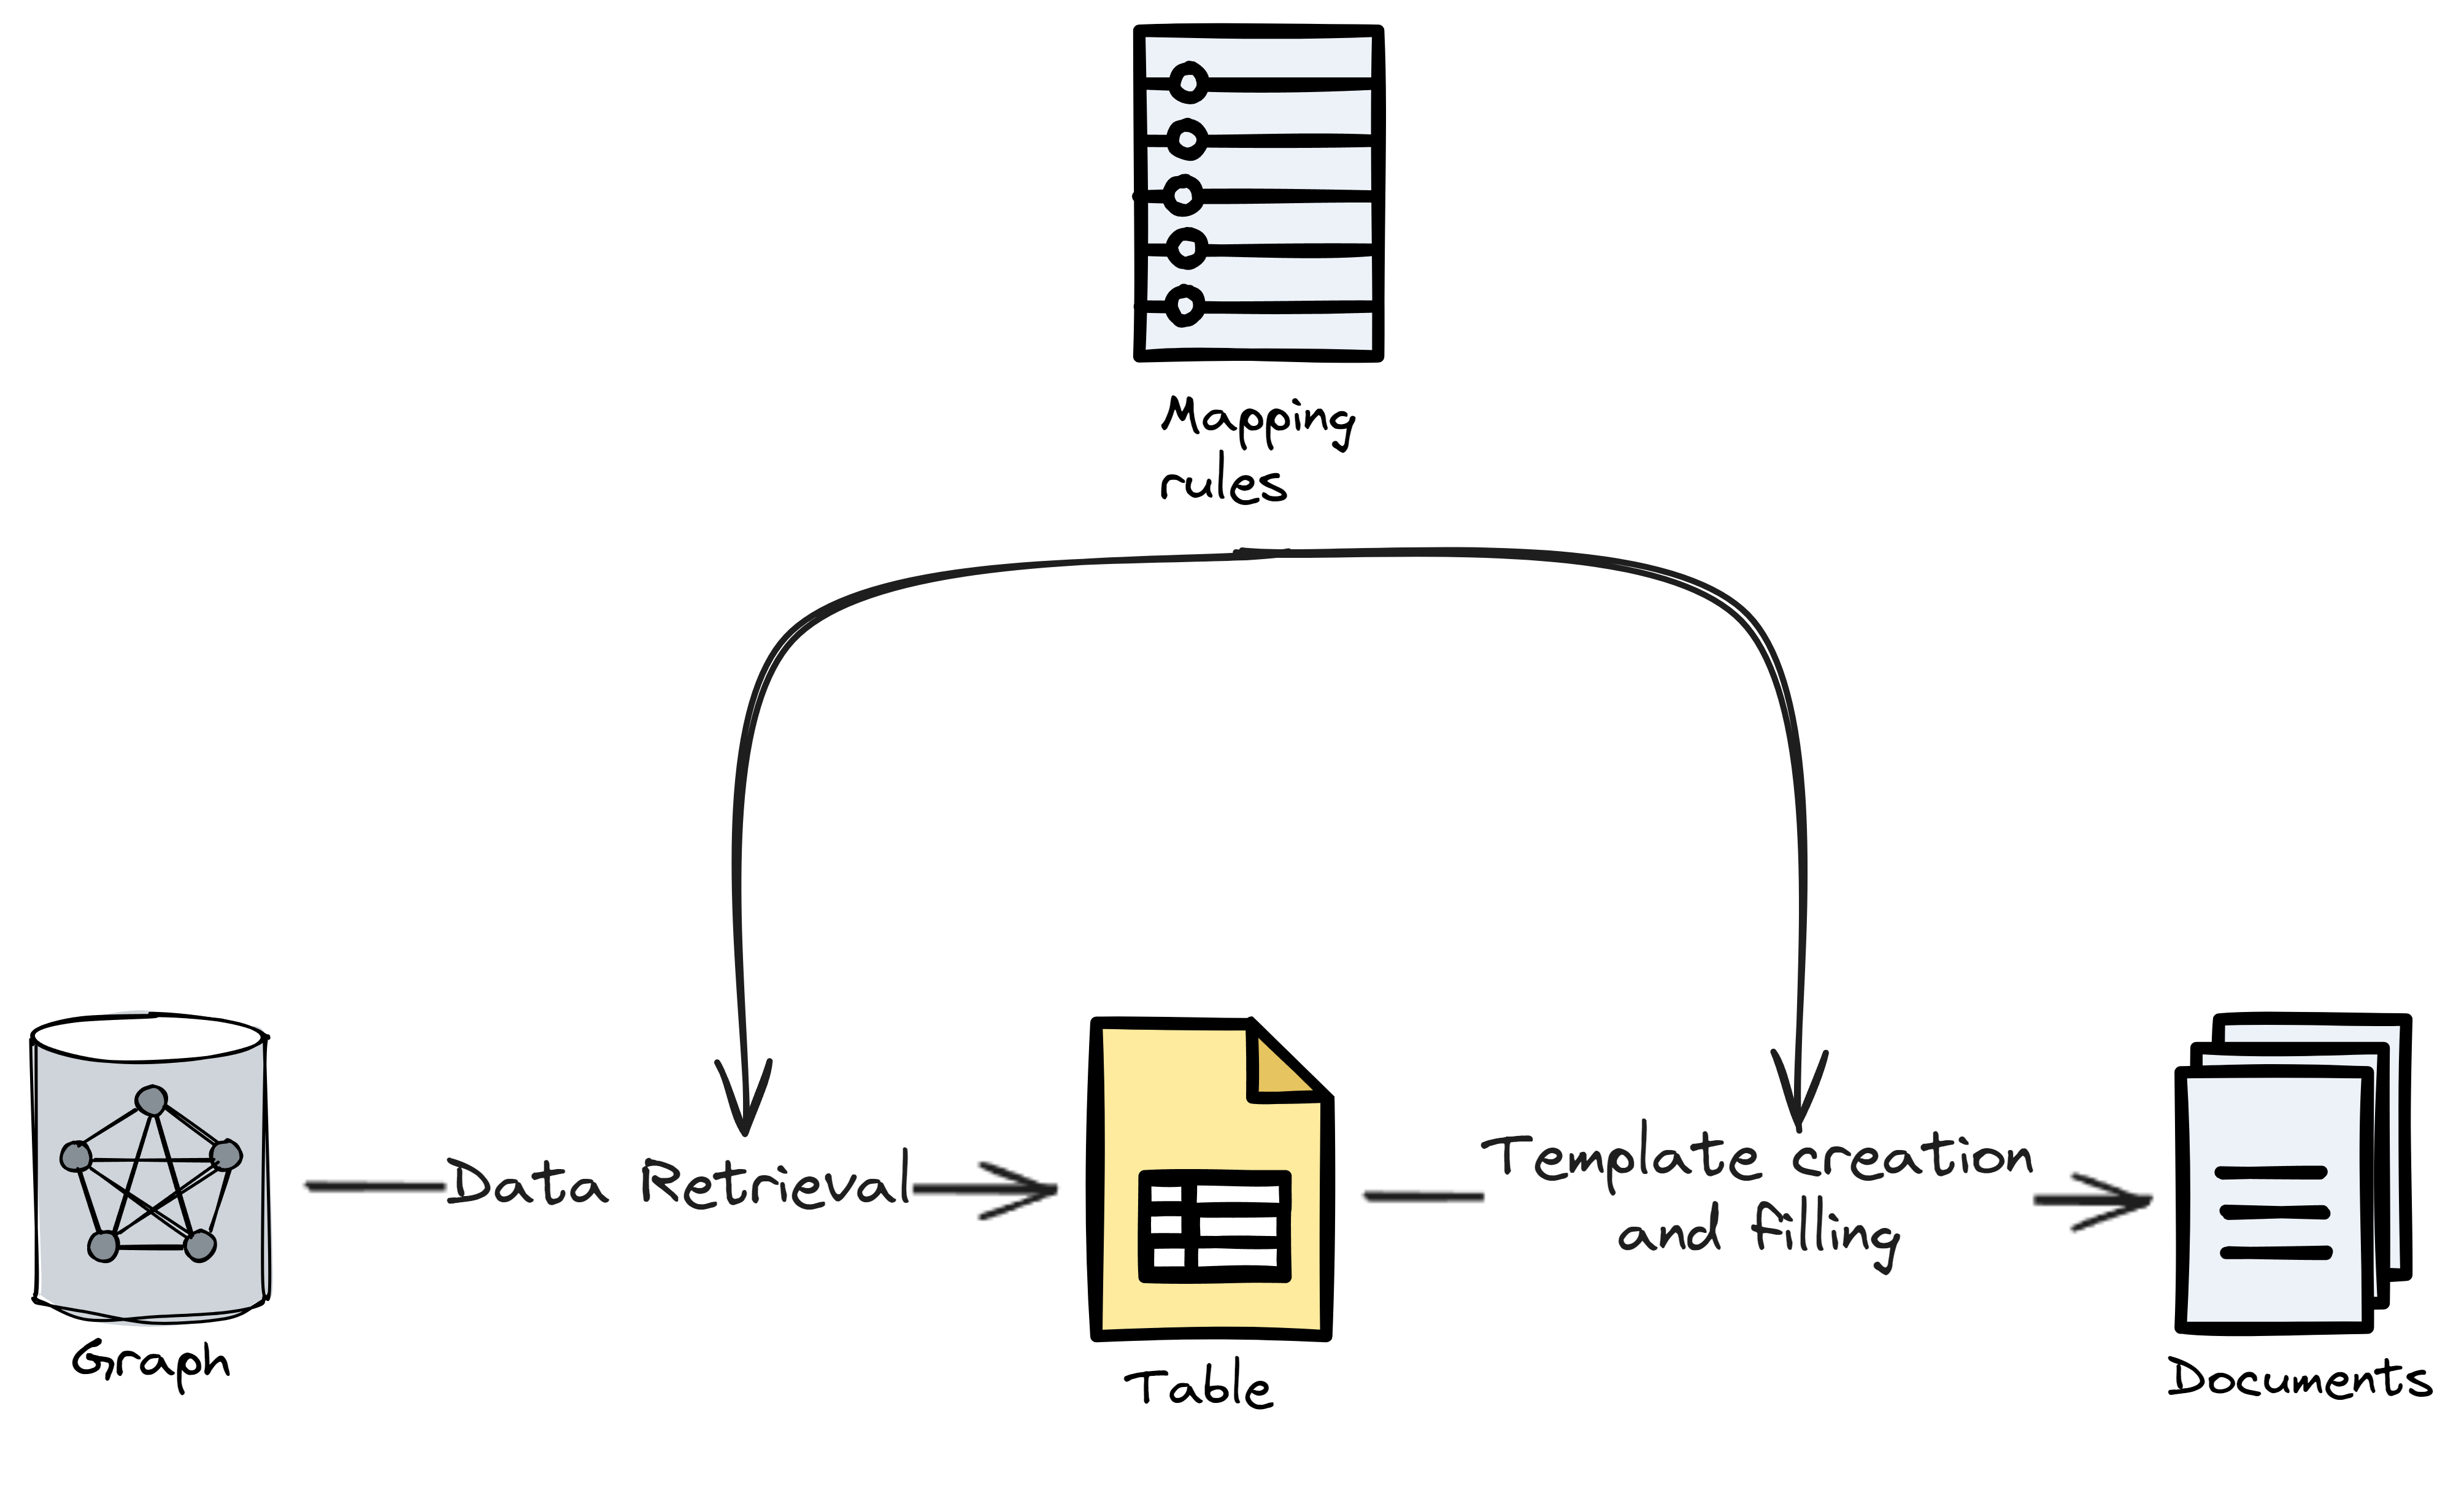
\includegraphics[width=0.9\textwidth]{fig/design.png}
    \caption{Design of the proposed system}
    \label{fig:design}   
\end{figure}


% At this time we only have a PoC implementation, as such many details haven't been worked out yet. For example, the section on creating the schema is limited, as we only handle CSV files which require little to no schema. 

\section{Setup}

We choose to make our implementation in Python as it both has an extensive set of libraries and is well suited for rapid development. We use Morph-KGC to process the mapping rules for its ease of use, being well made and its use of the pandas library to represent the mapping rules. As the graph source we choose a standalone SPARQL endpoint on a triple store. For working with graph(\acrshort{rdf}) files, we first upload them to a triple store.

First the endpoint is set up, if necessary. If the source is a file, it is uploaded to the endpoint using the SPARQL 1.1 Graph Store HTTP Protocol. In our setup this is a locally running the free version of GraphDB. The url of the repository is then wrapped using the SPARQLWrapper library and some settings are set.

Next we load the mapping rules from the mapping(\acrshort{rml}) files using Morph-KGC's internal \texttt{retrieve\_mappings} function. This function takes a config file (.ini format) as input, which specifies the location of the mapping files and various other settings which can be used to configure the behavior of the mapping. The mappings are returned as a pandas DataFrame which we enrich with various helper columns. An example of a single mapping rule (row in the DataFrame) can be found in listing \ref{lst:mapping_rule}. Marked in bold are the helper columns we add.

\begin{lstlisting}[caption={Example of a mapping rule in Morph-KGC}, label={lst:mapping_rule}, captionpos=b, basicstyle=\small]
source_name: DataSource1
triples_map_id: #TM0
triples_map_type: http://w3id.org/rml/TriplesMap
logical_source_type: http://w3id.org/rml/source
logical_source_value: student.csv
iterator: nan
subject_map_type: http://w3id.org/rml/template
subject_map_value: http://example.com/{Name}
[*subject_references_template: http://example.com/([^\/]*)$*]
[*subject_references: ['Name']*]
[*subject_reference_count: 1*]
subject_termtype: http://w3id.org/rml/IRI
predicate_map_type: http://w3id.org/rml/constant
predicate_map_value: http://xmlns.com/foaf/0.1/name
[*predicate_references_template: None
predicate_references: []
predicate_reference_count: 0*]
object_map_type: http://w3id.org/rml/reference
object_map_value: Name
[*object_references_template: None
object_references: ['Name']
object_reference_count: 1*]
object_termtype: http://w3id.org/rml/Literal
object_datatype: nan
object_language: nan
graph_map_type: http://w3id.org/rml/constant
graph_map_value: http://w3id.org/rml/defaultGraph
subject_join_conditions: nan
object_join_conditions: nan
source_type: CSV
mapping_partition: 1-1-1-1
\end{lstlisting}

\section{Retrieving the data}
\label{section:retrieving_data}
Retrieving the data is done by querying the \acrshort{sparql} endpoint using an automatically generated query. All the required data from the source is retrieved at once. This does result in some degree of duplication for nested structures, but doing all processing and joining server-side is preferable. This also has a disadvantage in disjointed mappings resulting in a Cartesian product of the fragments. This is further discussed in subsection \ref{subsection:disjointed_mappings}. The data is returned as a CSV-table which is then loaded into a pandas DataFrame for further processing. The only post processing done at the moment is the decoding of url-encoded strings where necessary. 

\subsection{Generating the queries}
\label{subsection:generating_queries}
To generate the queries we first select the triple maps we want to use to generate the query. While constant values are always included, sometimes we can lighten the load on the server by reducing the amount and complexity of mapping rules we use. We design three operating modes:
\begin{itemize}
    \item \textbf{Full}: All triple maps are used to generate the query. This is guaranteed to give predicatable results as it checks each instance of a mapped value.
    \item \textbf{Reduced}: All triple maps with a object map type of reference are used to generate the query. Only where necessary to retrieve all data template map types are used.
    \item \textbf{Minimal}: Only a single datapoint is used for each reference, with a preference for reference object map types.
\end{itemize}

We then generate the queries by translating the mapping rules into patterns. 
Each of the three map types, constant, reference, and template, generates a different pattern.
For the constant map type, we know that it will always be present with a constant value, so we can simply add it as a triple pattern like \texttt{?s a foaf:Person .}. 
Both reference and template map types will not generate a triple during materialization if any of the references are not present during the generation. We must take this into account by allowing for blank fields using the optional keyword.
Reference maps are the easiest to work with as they directly translate back to the source. An example of a basic query using constant and reference maps can be found in listing \ref{lst:simple_query_example}.

\begin{lstlisting}[caption={Simple query example}, label={lst:simple_query_example}, captionpos=b]
SELECT DISTINCT ?Name ?ID
WHERE {
    ?s a foaf:Person .

    optional{
        ?s foaf:name ?Name .
    }
    optional{
        ?s ex:id ?ID .
    }
}
\end{lstlisting}    

Template maps are the most complex to work with as their structure can wildly vary. The simplest step we can take is to confirm the mapped value matches with the map template like
\texttt{FILTER(regex(str(?s), "http://example.com/([\textasciicircum\textbackslash\textbackslash/]*)/([\textasciicircum\textbackslash\textbackslash/]*)\$"))}. Taking this further we can use string manipulation to split the variable into the different references. An example of this can be found in listing \ref{lst:template_query_example}.

\begin{lstlisting}[caption={Template query example}, label={lst:template_query_example}, captionpos=b]
SELECT DISTINCT ?Name ?ID
WHERE {
    ?s a foaf:Person .
    FILTER(regex(str(?s), "http://example\\.com/([^\\/]*)/([^\\/]*)$")) .
    BIND(STRAFTER(str(?s), "http://example.com/") as ?temp) .
    BIND(STRBEFORE(str(?temp), "/") as ?ID)
    BIND(STRAFTER(?temp, "/") as ?Name)

    optional{
        ?s foaf:name ?Name .
    }
    optional{
        ?s ex:id ?ID .
    }
}
\end{lstlisting}

The algorithm for generating the queries can be found in algorithm \ref{alg:generate_query}. This is still an early version of the algorithm, which needs to be improved to handle more complex mappings.

\begin{algorithm} 
    \caption{Generating the queries}
    \label{alg:generate_query}
    \begin{algorithmic}[1]
        \Require{$iterator$ is the iterator to generate the query for}
        \Require{$mapping\_rules$ is a set of mapping rules for said iterator}
        \State $query\_lines \gets []$
        \ForAll{$rule \in mapping\_rules$}
            \If{$rule.is\_constant()$}
                \State $query\_lines.append(rule.to\_triple())$ 
            \ElsIf{$rule.is\_reference()$}
                \State $query\_lines.append(rule.to\_optional\_triple())$
            \ElsIf{$rule.is\_template()$}
                \State $query\_lines.append(test\_object\_regex(rule))$
                \State $remainder \gets rule['object\_map\_value']$
                \ForAll{$reference \in rule['object\_references']$}
                    \State $query\_lines.append(bind_reference_part(rule, reference))$
                \EndFor
            \EndIf
        \EndFor
        \State $query \gets wrap\_query\_lines(query\_lines)$
    \end{algorithmic}
\end{algorithm}

\subsection{Disjointed mappings}
\label{subsection:disjointed_mappings}

We generate a single query for each iterator. This query can contain multiple subjects. This can, however, lead to issues when the subjects share no references. The effect we get is not unlike joining two tables in SQL without join conditions. For example, using the mapping listed in listing \ref{lst:bad_join_example} we get the query in listing \ref{lst:bad_join_query}. When applied to the knowledge graph in listing \ref{lst:bad_join_kg} we get the result in listing \ref{lst:bad_join_result} instead of the original source in listing \ref{lst:bad_join_expected_result}. When converting the badly generated source back to the knowledge graph, we do get the same knowledge graph as the original as the duplicate data is ignored. The amount of duplicate data increases exponentially with the number of subjects so even though ignoring it would be a valid solution, it is not viable with larger datasets. The only solution to this problem is updating the mapping rules to either split the source or add shared references. The user is ultimately responsible for this, but we could generate a warning to notify the user. 

\begin{listing}
    \refstepcounter{lstlisting}
    \noindent\begin{minipage}[b]{.45\textwidth}
        \begin{lstlisting}[basicstyle=\small]
<TriplesMap1> a rr:TriplesMap;
rml:logicalSource [ 
    rml:source "student_sport.csv";
    rml:referenceFormulation ql:CSV
];
rr:subjectMap [ 
    rr:template "http://example.com/{Student}";
    rr:class ex:Student
];
rr:predicateObjectMap [ 
    rr:predicate foaf:name ; 
    rr:objectMap [ 
        rml:reference "Student"
    ]
].
        \end{lstlisting}      
    \end{minipage}
    \hfill
    \begin{minipage}[b]{.45\textwidth}
        \begin{lstlisting}[basicstyle=\small]
<TriplesMap2> a rr:TriplesMap;
rml:logicalSource [ 
    rml:source "student_sport.csv";
    rml:referenceFormulation ql:CSV
];
rr:subjectMap [ 
    rr:template "http://example.com/{Sport}";
    rr:class ex:Sport
];
rr:predicateObjectMap [ 
    rr:predicate foaf:name ; 
    rr:objectMap [ 
        rml:reference "Sport"
    ]
].
        \end{lstlisting}
    \end{minipage}
    \addtocounter{listing}{5}
    \caption{Bad join mapping}
    \label{lst:bad_join_example}
\end{listing}

\begin{lstlisting}[caption={Bad join query (trimmed)}, label={lst:bad_join_query}, captionpos=b, basicstyle=\small]






SELECT DISTINCT ?Student_name ?Sport
WHERE {
    ?s1 a ex:Student .
    optional{
        ?s1 foaf:name ?Student_name .
    }
    ?s2 a ex:Sport .
    optional{
        ?s2 foaf:name ?Sport .
    }
}
\end{lstlisting}

\begin{lstlisting}[caption={Bad join knowledge graph}, label={lst:bad_join_kg}, captionpos=b, basicstyle=\small]
@prefix ex: <http://example.com/> .
@prefix foaf: <http://xmlns.com/foaf/0.1/> .

ex:Venus a ex:Student ;
    foaf:name "Venus" .
ex:Tom a ex:Student ;
    foaf:name "Tom" .
ex:Tennis a ex:Sport ;
    foaf:name "Tennis" .
ex:Football a ex:Sport ;
    foaf:name "Football" .
\end{lstlisting}

\begin{lstlisting}[caption={Bad join result}, label={lst:bad_join_result}, captionpos=b, basicstyle=\small]
Student,Sport
Venus,Tennis
Venus,Football
Tom,Tennis
Tom,Football
\end{lstlisting}

\begin{lstlisting}[caption={Bad join original source}, label={lst:bad_join_expected_result}, captionpos=b]
Student,Sport
Venus,Tennis
Tom,Football
\end{lstlisting}

\section{Contructing the schema}
\label{section:constructing_schema}
Constructing the schema is done by reversing the mapping rules' source. We do this using the iterator and the mapping rule's references. \acrshort{rml} supports many different types of sources and referenceFormulations. We will implement the CSV, xPath, and JSONPath referenceFormulations. Not every source is a file, so for query-based sources, we will generate the query output. In a later stage, we could look into taking it a step further, generating the actual source behind those intermediate results.

As each referenceFormulation has its reference syntax, we will have to tailor the implementation to each referenceFormulation. For the PoC, we only implement the CSV referenceFormulation. 

\subsection{CSV}
\label{subsection:csv}
The CSV referenceFormulation is the simplest of the three as it describes a simple two-dimensional table, with columns having the names of the references and rows being the iterated values. The example TriplesMap in listing \ref{lst:csv_file_mapping} results in the CSV template in listing \ref{lst:csv_file}. Unlike the other referenceFormulations, CSV has no uncertainty in terms of structure.

\begin{lstlisting}[caption={Example mapping for a CSV file}, label={lst:csv_file_mapping}, captionpos=b, basicstyle=\small]
<TriplesMap1> a rr:TriplesMap;

rml:logicalSource [ 
    rml:source "student.csv";
    rml:referenceFormulation ql:CSV
];

rr:subjectMap [ 
    rr:template "http://example.com/Student/{ID}/{Name}";
    rr:graph ex:PersonGraph ;
    rr:class foaf:Person
];

rr:predicateObjectMap [ 
    rr:predicate ex:id ; 
    rr:objectMap [ rml:reference "ID" ]
];

rr:predicateObjectMap [ 
    rr:predicate foaf:name ; 
    rr:objectMap [ rml:reference "Name" ]
].
\end{lstlisting}

\begin{lstlisting}[caption={Example CSV template}, label={lst:csv_file}, captionpos=b, basicstyle=\small]
[*ID,Name*]
<ID>,<Name>
\end{lstlisting}

\section{Applying the data to the schema}
\label{section:applying_data}
Generating the final output is done by iterating over the rows of the data and applying them to the schema. Each column of the data corresponds to a reference in the schema. A short version of the algorithm can be found in algorithm \ref{alg:apply_data}. For the PoC this approach is sufficient, even too complex as we can simply dump the query-result DataFrame to a CSV file. For more complex, possibly nested, sources we will have to adapt this algorithm.

\begin{algorithm}
    \caption{Applying the data to a simple (non-nested) schema}
    \label{alg:apply_data}
    \begin{algorithmic}[1]
        \Require{$schema$ is a schema}
        \Require{$data$ is a DataFrame}
        \State $output \gets new\_file$
        \ForAll{$row \in data$}
            \State $output \gets schema$
            \ForAll{$column \in row$}
                \State $schema.replace(column.name, column.value)$
            \EndFor
            \State $output.write(schema)$
        \EndFor
    \end{algorithmic}
\end{algorithm}

%%%%%%%%%%%%%%%%%%%%%%%%%%%%%%%%%%%%%%%%%%%%%%%%%%%%%%%%%%%%%%%%%%% 
%                                                                 %
%                            CHAPTER                              %
%                                                                 %
%%%%%%%%%%%%%%%%%%%%%%%%%%%%%%%%%%%%%%%%%%%%%%%%%%%%%%%%%%%%%%%%%%% 
\chapter{Evaluation}
\label{chapter:evaluation}
In this chapter we will evaluate our implementation. We will do this by testing it again various datasets, comparing the expected results with the actual results. For each dataset we will go over our testing methodology and its results. For the PoC implementation we only test the RML test cases. 

Please note that the implementation for the results uses an earlier version of the algorithm, as we did not have time to update the implementation to the current version of the algorithm. As the updates to the algorithm were largely to solve to the failed test cases, we expect the results to be better if we had time to update the implementation.

\section{RML test cases}
\label{section:rml_test_cases}
The RML test cases are a set of test cases to evaluate the conformity of an RML processor. Though these test cases are not a perfect match, they offer expected outputs for certain inputs and mapping rules, making them a good starting point for testing our implementation. The test cases are designed with edge cases in mind, making them a good set of test cases to test a mapper. Using them to test inversion, however, is stretching their purpose a bit. As such we have to filter out test cases that are expected to fail, as they do not produce a result. As the reading of the mappings is handled by Morph-KGC, some test cases that test things like alternative syntax look the same to us, providing little value.

In table \ref{tab:rml_test_cases} the results of the RML test cases can be found. The failed tests are divided into categories with colours according to the reason they failed. The red failures are caused by solvable issues in the implementation. The orange failure is caused by disconnected subjects in a single iterator, as such no solution is planned for this. The light-red failures are because of limitations of the Morph-KGC library. 

\begin{table}[]
    \centering
    \begin{tabular}{ll
    >{\columncolor[HTML]{FFFFFF}}l ll}
    Test                              & Status                         & {\color[HTML]{000000} } & Test                              & Status                         \\
    \cellcolor[HTML]{00FF00}0000-CSV  & \cellcolor[HTML]{00FF00}\cmark & {\color[HTML]{000000} } & \cellcolor[HTML]{00FF00}0008a-CSV & \cellcolor[HTML]{00FF00}\cmark \\
    \cellcolor[HTML]{00FF00}0001a-CSV & \cellcolor[HTML]{00FF00}\cmark & {\color[HTML]{000000} } & \cellcolor[HTML]{FF0000}0008b-CSV & \cellcolor[HTML]{FF0000}\xmark \\
    \cellcolor[HTML]{00FF00}0001b-CSV & \cellcolor[HTML]{00FF00}\cmark & {\color[HTML]{000000} } & \cellcolor[HTML]{00FFFF}0008c-CSV & \cellcolor[HTML]{00FFFF}\xmark \\
    \cellcolor[HTML]{00FF00}0002a-CSV & \cellcolor[HTML]{00FF00}\cmark & {\color[HTML]{000000} } & \cellcolor[HTML]{FF0000}0009a-CSV & \cellcolor[HTML]{FF0000}\xmark \\
    \cellcolor[HTML]{00FF00}0002b-CSV & \cellcolor[HTML]{00FF00}\cmark & {\color[HTML]{000000} } & \cellcolor[HTML]{FF0000}0009b-CSV & \cellcolor[HTML]{FF0000}\xmark \\
    \cellcolor[HTML]{00FF00}0003c-CSV & \cellcolor[HTML]{00FF00}\cmark & {\color[HTML]{000000} } & \cellcolor[HTML]{00FFFF}0010a-CSV & \cellcolor[HTML]{00FFFF}\xmark \\
    \cellcolor[HTML]{FF9900}0004a-CSV & \cellcolor[HTML]{FF9900}\xmark & {\color[HTML]{000000} } & \cellcolor[HTML]{00FFFF}0010b-CSV & \cellcolor[HTML]{00FFFF}\xmark \\
    \cellcolor[HTML]{00FFFF}0005a-CSV & \cellcolor[HTML]{00FFFF}\xmark & {\color[HTML]{000000} } & \cellcolor[HTML]{FF0000}0010c-CSV & \cellcolor[HTML]{FF0000}\xmark \\
    \cellcolor[HTML]{00FFFF}0006a-CSV & \cellcolor[HTML]{00FFFF}\xmark & {\color[HTML]{000000} } & \cellcolor[HTML]{00FFFF}0011b-CSV & \cellcolor[HTML]{00FFFF}\xmark \\
    \cellcolor[HTML]{00FFFF}0007a-CSV & \cellcolor[HTML]{00FFFF}\xmark & {\color[HTML]{000000} } & \cellcolor[HTML]{00FFFF}0012a-CSV & \cellcolor[HTML]{00FFFF}\xmark \\
    \cellcolor[HTML]{00FFFF}0007b-CSV & \cellcolor[HTML]{00FFFF}\xmark & {\color[HTML]{000000} } & \cellcolor[HTML]{FF0000}0012b-CSV & \cellcolor[HTML]{FF0000}\xmark \\
    \cellcolor[HTML]{FF0000}0007c-CSV & \cellcolor[HTML]{FF0000}\xmark & {\color[HTML]{000000} } & \cellcolor[HTML]{FF0000}0015a-CSV & \cellcolor[HTML]{FF0000}\xmark \\
    \cellcolor[HTML]{FF0000}0007d-CSV & \cellcolor[HTML]{FF0000}\xmark & {\color[HTML]{000000} } & \cellcolor[HTML]{EA9999}0019a-CSV & \cellcolor[HTML]{EA9999}\xmark \\
    \cellcolor[HTML]{00FF00}0007e-CSV & \cellcolor[HTML]{00FF00}\cmark & {\color[HTML]{000000} } & \cellcolor[HTML]{EA9999}0019b-CSV & \cellcolor[HTML]{EA9999}\xmark \\
    \cellcolor[HTML]{00FFFF}0007f-CSV & \cellcolor[HTML]{00FFFF}\xmark & {\color[HTML]{000000} } & \cellcolor[HTML]{00FF00}0020a-CSV & \cellcolor[HTML]{00FF00}\cmark \\
    \cellcolor[HTML]{00FFFF}0007g-CSV & \cellcolor[HTML]{00FFFF}\xmark & {\color[HTML]{000000} } & \cellcolor[HTML]{EA9999}0020b-CSV & \cellcolor[HTML]{EA9999}\xmark
    \end{tabular}
    \captionsetup{justification=centering}
    \caption{Results of the RML test cases}
    \label{tab:rml_test_cases}
\end{table}
%%%%%%%%%%%%%%%%%%%%%%%%%%%%%%%%%%%%%%%%%%%%%%%%%%%%%%%%%%%%%%%%%%% 
%                                                                 %
%                            CHAPTER                              %
%                                                                 %
%%%%%%%%%%%%%%%%%%%%%%%%%%%%%%%%%%%%%%%%%%%%%%%%%%%%%%%%%%%%%%%%%%% 
\chapter{Conclusion}
\label{chapter:conclusion}
In this master thesis we explored the possibility of inverting knowledge graphs back to their original raw data format using mapping rules. To this end we created a generic two-module design and made an implementation using RML mapping rules. We implemented a data retrieval module using SPARQL and two templating modules for CSV and JSON. 

The data retrieval module takes the knowledge graph, either a file or an endpoint, and uses the mapping rules to retrieve the data from it. In our case it translates selected triple maps in the mapping rules to parts of a SPARQL query, adapting the approach based on the type of the triple map. The selection process aims to balance performance and reliability. Generating the output is made more challenging by the requirement to handle both absent fields and multiple occurrences of the same field while ensuring their equality. We found that to ensure proper inversion we cannot use the full RML specification, but must impose restrictions on the mapping rules. These restrictions pertain to the access of the source and transformation of the data. 
To fully reconstruct a data source no aggregation, filtering or other irreversible transformations on the source can be done. Additionally, the mapping must use all the data in the source. 
In order to be able to reconstruct values of the data, no possibly irreversible transformations can be done on them, as any information lost during a lossy transformation is impossible to regain. This includes the use of templates, where the divider between different references cannot be present in the references. \acrshort{uri} encoded templates are an exception, here the transformation is guaranteed to be reversible if reserved characters are used as divider.

The templating module takes the data retrieved by the data retrieval module and uses it to create the source file. In case of the CSV templating module this is a simple process, as the data is already in the correct format. The JSON templating module is more complex, as JSON has a nested structure. We take all the paths from which data is retrieved and create a template from them. This template is then recursively filled from the root node, splitting the data at each array. To properly create the JSON template all filepaths must be linearly connected to the root node, using JSON features like recursive descent makes the path taken to the data unclear and the template impossible to create. This is another restriction we must impose on the mapping rules.

We evaluated our implementation using the RML test cases to test various edge cases, the LUBM4OBDA benchmark to test the scalability of our data retrieval module and the GTFS-Madrid benchmark to evaluate the performance of the JSON templating module. We find that our implementation is able to invert the knowledge graph back to the original source files in most cases. The failures are mostly due to limitations of the mapping processor, incompatible mapping rules or different data representations. The LUBM4OBDA benchmark shows that our data retrieval module scales linearly with the size of the knowledge graph and is completely dependent on the power of the SPARQL endpoint. The GTFS-Madrid benchmark shows that the JSON templating module also scales linearly with the size of the knowledge graph.

\section{Future work}
In this section we will discuss possible future work that can be done to expand on our implementation. The implementation can be expanded on in both depth and breadth. 

\subsection{Functions}
RML offers the capability to transform data using functions with the Function Ontology (FnO). Expanding the capabilities of the data retrieval module to encompass this is a possible next step. Functions that merely transform data without losing information could be directly inverted. The data lost in lossy transformations could in some cases be regained by calling on an external data source. Lastly lossy functions could be used to verify the correctness of data values with duplicate references of which one was run through a lossy function.

Implementing this would expand the depth of the implementation. We did not implement it due to the large complexity and time to implement it compared to the limited benefits it is expected to provide.

\subsection{Additional templating modules}
We created two templating modules, one for CSV and one for JSON. Each a representative of a different type of data format: tabular and nested. Creating additional templating modules would make the implementation more versatile, further allowing mixed data formats in mappings. 

A special case where we don't recreate the data source would be to make a database update module. If the primary key of a table is present in the references an update query could be made to update the database. 


% Eventueel enkele appendices
%%%%%%%%%%%%%%%%%%%%%%%%%%%%%%
%\appendix

% Bibliografie: referenties. De items zitten in bibliografie.bib
%%%%%%%%%%%%%%%%%%%%%%%%%%%%%%%%%%%%%%%%%%%%%%%%%%%%%%%%%%%%%%%%%
% Indien je ook de niet geciteerde werken in je bibliografie wil opnemen, commentarieer dan onderstaande regel uit!
\nocite{*}
\bibliographystyle{apalike}
\bibliography{bibliografie}

\end{document}

% Back cover: change according to the correct campus

\includepdf{private/back_fiiw_denayer_eng.pdf} % For the English version

% \end{document}